\documentclass[11pt]{article}
\usepackage[utf8]{inputenc} % Para caracteres en espa�ol
\usepackage{amsmath,amsthm,amsfonts,amssymb,amscd}
\usepackage{multirow,booktabs}
\usepackage[table]{xcolor}
\usepackage{fullpage}
\usepackage{lastpage}
\usepackage{enumitem}
\usepackage{multicol}
\usepackage{fancyhdr}
\usepackage{mathrsfs}
\usepackage{wrapfig}
\usepackage{setspace}
\usepackage{esvect}
\usepackage{calc}
\usepackage{multicol}
\usepackage{cancel}
\usepackage{graphicx}
\graphicspath{ {pictures/} }
\usepackage[retainorgcmds]{IEEEtrantools}
\usepackage[margin=3cm]{geometry}
\usepackage{amsmath}
\newlength{\tabcont}
\setlength{\parindent}{0.0in}
\setlength{\parskip}{0.05in}
\usepackage{empheq}
\usepackage{framed}
\usepackage[most]{tcolorbox}
\usepackage{xcolor}
\colorlet{shadecolor}{orange!15}
\parindent 0in
\parskip 12pt
\geometry{margin=1in, headsep=0.25in}
\theoremstyle{definition}
\newtheorem{defn}{Definition}
\newtheorem{reg}{Rule}
\newtheorem{exer}{Exercise}
\newtheorem{note}{Note}
\newcommand{\volume}{{\ooalign{\hfil$V$\hfil\cr\kern0.08em--\hfil\cr}}}
\newcommand{\parr}{\mathbin{\|}} % Parralel Symbol
\begin{document}
\setcounter{section}{2}
\setcounter{page}{25}
\setcounter{equation}{49}

 \pagestyle{fancy}
\fancyhf{}
\rhead{Section 2: Electromagnetics}
\rfoot{Page \thepage}
\thispagestyle{empty}


\begin{center}
{\LARGE \bf Section 2: Electromagnetics}\\
{\large AE435}\\
Spring 2018
\end{center}
In this section, we will review the basics of charge, electricity, magnetism, and Maxwell equations.
\vspace{25mm}
\section{Magnetostatics}
\begin{center}
"Charge in motion creates a magnetic field"
\end{center}
\tableofcontents
\newpage
\subsection{Electric Current}
\begin{shaded}
\textbf{Current} \newline
\begin{equation}
J \equiv \frac{\partial Q}{\partial t} \qquad \bigg[\frac{c}{s}\bigg] = \big[A\big] = \text{Amps}
\end{equation}
\end{shaded}
We'll use J, although sometimes we see I used for current. Currents can flow in a range of media: metals, semiconductors, fluids, gases and plasmas.

\textbf{METALS}
\newline
In metals, there are fixed ionic cores with bound inner ions:
\begin{center}
\vfill
\textbf{Figure 12}
\end{center}
Outer valence electrons get freely traded from ion to ion in response to electric fields. In other words, say we put  10 electrons in one end of a wire and we get 10 electrons out the other end. Those won't be the same 10 electrons we put in though.

\textbf{GASES AND PLASMAS}
\newline
In gases and plasmas, both electrons AND ions move:
\begin{center}
\vfill
\textbf{Figure 13}
\end{center}
\begin{itemize}
\item Most of the conduction is by electrons, because they're much lighter.
\item In thermal motion, both ions and electrons are as likely to cross plane in one direction as another, so no net current.
\item Under electric field, drift velocity of species (ions toward cathode, electrons toward anode) gives rise to current.
\end{itemize}
\newpage
\subsection{Current Density}
Consider flux of particles through surface element dS:
\begin{center}
\vfill
\textbf{Figure 14}
\end{center}
Since particle with charge q crossing dS carries incremental current $q \, \vv{v} \cdot \hat{n}$. For N particles per unit volume, current crossing dS is then:
\begin{equation*}
\begin{aligned}
\mathrm{d}J = N \, q \, \vv{v} \cdot \hat{n} \, \mathrm{d}S
\end{aligned}
\end{equation*}
For multiple species, sum over all:
\begin{equation*}
\begin{aligned}
\mathrm{d}J = \sum_i N_i \, q_i \, \vv{v}_i \cdot \hat{n} \, \mathrm{d}S
\end{aligned}
\end{equation*}
Define current density as a vector current per unit area:
\begin{shaded}
\textbf{Current Density} \newline
\begin{equation}
\vv{j} = \sum_i N_i \, q_i \, \vv{v}_i \qquad \bigg[\frac{A}{m^2}\bigg]
\end{equation}
\end{shaded}
So, the total current across a surface S is:
\begin{shaded}
\textbf{Total Current Across a Surface} \newline
\begin{equation}
J = \int_S \vv{j} \cdot \hat{n} \, \mathrm{d}S
\end{equation}
\end{shaded}
\newpage
\subsection{Continuity}
Consider volume $\volume$ enclosed by surface S, within a current density field
\begin{center}
\vspace{70mm}
\textbf{Figure 15}
\end{center}
Current crossing in or out of $\volume$ through S is:
\newline \newline
\begin{equation}
\begin{aligned}
J = \int_S \vv{j} \cdot \hat{n} \, \mathrm{d}S = \int_{\volume} \nabla \cdot \vv{j} \, \mathrm{d}\volume
\end{aligned}
\end{equation}
\newline \newline
Note that positive current refers to what is going into the volume.
\newline
\newline
We also know from the definition of current (Equation 50), and from definition of volume charge density, and for a steady control volume:
\newline \newline
\begin{equation}
\begin{aligned}
J = \frac{\partial Q}{\partial t} = \frac{\mathrm{d}}{\mathrm{d}t}\int_{\volume} \rho_e \, \mathrm{d}\volume = \int_{\volume} \frac{\partial\rho_e}{\partial t} \, \mathrm{d}\volume
\end{aligned}
\end{equation}
\newline \newline
Combining Equation 54 and Equation 53, we get:
\newline \newline
\begin{equation*}
\begin{aligned}
\int_{\volume} \bigg( \frac{\partial \rho_e}{\partial t} + \nabla \cdot \vv{j} \bigg) \, \mathrm{d}\volume = 0
\end{aligned}
\end{equation*}
\newline
\newpage
This must be true for any arbitrary volume, therefore the
integrand must vanish at every point, giving:
\begin{shaded}
\textbf{Continuity: Conservation of Charge} \newline
\begin{equation}
\frac{\partial \rho_e}{\partial t} + \nabla \cdot \vv{j} = 0
\end{equation}
Where:
\begin{equation*}
\begin{split}
\rho_e &= \text{Charge density} \\ \\
\frac{\partial \rho_e}{\partial t} &= \text{Time rate of change of some quantity within the volume} \\ \\
\nabla \cdot \vv{j} &= \text{The cause for that quantity to change with time} \\ \\
\end{split}
\end{equation*}
\end{shaded}
The right hand side being equal to zero tells us that nothing else can change the continuity. If the right hand side were to not equal zero, then we would be describing a case where something is changing. For the case of charge, that could be a chemical reaction that changes how continuity behaves.
\newline \newline
Sometimes, it may be beneficial to recall how continuity was described in terms of fluid dynamics.
\newpage
\subsection{Ohm's Law}
Experiments show that
\begin{shaded}
\textbf{Ohm's Law} \newline
\begin{equation}
\vv{j} = \sigma (\vv{E}) \, \vv{E}
\end{equation}
Where:
\begin{equation*}
\begin{split}
\vv{j} &= \text{Current} \\
\sigma (\vv{E}) &= \text{Conductivity} \\
\vv{E} &= \text{Description} \\
\end{split}
\end{equation*}
\end{shaded}
Where the conductivity, $\sigma$, has units of Siemens/m. Note that $\sigma$ is \textbf{NOT} the surface charge density! In common conductors (such as metals, electrolytes and unmagnetized plasmas) $\sigma (\vv{E}) = \sigma$ is a constant. These are called \textbf{linear media} or \textbf{ohmic media}. 
\newline \newline
If you take the reciprocal of the conductivity, you get the resistivity,
\begin{shaded}
\textbf{Resistivity} \newline
\begin{equation}
\sigma = \frac{1}{\rho} \qquad \Big[\text{Ohm-m}\Big]
\end{equation}
Where:
\begin{equation*}
\begin{split}
\rho  &= \text{Resistivity} \\
& \quad \rho \text{ is NOT volume change density}\\
\end{split}
\end{equation*}
\end{shaded}
For steady currents, $\frac{\partial \rho_e}{\partial t} = 0$. By continuity
then:
\newline
\begin{equation}
\begin{aligned}
\nabla \cdot \vv{j} = 0
\end{aligned}
\end{equation}
\newline
Now substituting in conductivity:
\newline
\begin{equation}
\begin{aligned}
\nabla \cdot \sigma \, \vv{E} = 0
\end{aligned}
\end{equation}
\newline
For a homogeneous media, meaning it has constant $\sigma$ over space:
\newline
\begin{equation}
\begin{aligned}
\nabla \cdot \vv{E} = 0
\end{aligned}
\end{equation}
\newline
which for electrostatic fields is just Laplace's Equation $\big( \vv{E} = - \nabla \phi \big)$
\newline
\begin{equation}
\begin{aligned}
\nabla^2 \phi = 0
\end{aligned}
\end{equation}
\newline
Given boundary conditions of $\phi$ or $\vv{j}$ at surfaces of a medium, we can solve for $\vv{j}$ in the medium.
\newline \newline
\underline{For Copper}, if we begin heating it (increasing its temperature), we see that
\begin{itemize}
\item Resistance \textbf{Increases}
\item Power required to heat \textbf{Increases}
\item Temperature \textbf{Increases}
\end{itemize}
And the cycle continues until it melts.
\newline \newline \newline \newline
\underline{For Plasma}, if we begin heating it (increasing its temperature), we see that
\begin{itemize}
\item Resistance \textbf{Decreases}
\item Power required to heat \textbf{Increases}
\item Temperature \textbf{Increases}
\end{itemize}
The resistance of plasma goes down as we heat it. This means that if we want to continue heating it, we must continue supplying more and more power.
\newpage
\subsection{Magnetic Field}
Recall the description of force on a charge, Coulomb's Law, from section II.1.
\newline
Once again, we will look at a \textbf{Two-Particle Model}:
\begin{center}
\vspace{70mm}
The force on q due to $q_1$ is Equation 1, $\vv{F}_e = \frac{1}{4 \, \pi \, \epsilon_0} \big( \frac{q \, q_1}{r^2}\big)\frac{\vv{r}}{r}$.
\newline
\newline
\textbf{Figure 16}
\end{center}
\newline
\newline
But what if the charges are moving? Let q move at a velocity $\vv{v}$ and $q_1$ move at a velocity $\vv{v}_1$. In this case, there's now another force on q due to $q_1$. This force is the \textbf{Magnetic Force.}
\newline
\newline
\begin{equation}
\begin{aligned}
\vv{F}_m = \frac{\mu_0}{4 \, \pi} \Big( \frac{q \, q_1}{r^2}\Big)\vv{v} \times \Big(\vv{v}_1 \times \frac{\vv{r}}{r}\Big)
\end{aligned}
\end{equation}
\newline
\newline
Where $\mu_0$ is the \textbf{Permeability of Free Space} and is proportional to:
\newline
\begin{equation}
\begin{aligned}
\frac{\mu_0}{4 \, \pi} &= 10^{-7} \qquad \Bigg[\frac{N \cdot s^2}{c^2}\Bigg] 
\end{aligned}
\end{equation}
\newline
\newline
By grouping the terms relating to the field charge $q_1$ , we can define a vector field that represents the force on the test charge q moving at velocity $\vv{v}_1$ such that:
\newline
\begin{equation*}
\begin{aligned}
\vv{F}_m = \frac{\mu_0}{4 \, \pi} \Big( \frac{q \, q_1}{r^2}\Big)\vv{v} \times \Big(\vv{v}_1 \times \frac{\vv{r}}{r}\Big)
\end{aligned}
\end{equation*}
\newpage
\begin{shaded}
\textbf{Magnetic Force}
\begin{equation}
\begin{aligned}
\vv{F}_m = q \, \vv{v} \times \vv{B}
\end{aligned}
\end{equation}
Where
\begin{equation}
\begin{split}
\vv{B} &= \frac{\mu_0}{4 \, \pi} \, \frac{q_1}{r^2} \, \Big(\vv{v}_1 \times \frac{\vv{r}}{r}\Big) \qquad \Bigg[\frac{N \, s}{c \, m}\Bigg] = [T]  \\ \\
\end{split}
\end{equation}
\end{shaded}
\newline
This vector field, $\vv{B}$, is the \underline{magnetic induction} which is the magnetic field intensity, and has SI units Tesla. Note: 1 Tesla $\approx$ 10,000 Gauss.
\newline
\newline
Therefore, the total force acting on test charge q is the combination of both the Electric AND Magnetic forces, which is called the Lorentz Force.
\newline
\begin{framed}
\textbf{Lorentz Force}
\begin{equation}
\begin{split}
\vv{F}_{\text{total}} = \vv{F}_{\text{E}} + \vv{F}_{\text{M}} = q \, \vv{E} + q \, \vv{v} \times \vv{B} = q \, \big(\vv{E} + \vv{v}\times\vv{B} \, \big)
\end{split}
\end{equation}
\end{framed}
\newline
Now lets consider, \textbf{What is the work done by a stationary magnetic field?}
\newline
\begin{equation*}
\begin{split}
\dot{W} = \vv{F}_{m} \cdot \vv{v} = q \, \vv{v} \times \vv{B} \cdot \vv{v} = 0
\end{split}
\end{equation*}
\newline
Essentially, a stationary magnetic field cannot do work/accelerate a fluid/particle/charge.
\newpage
\subsection{Forces on Conductors}
Consider a conducting circuit immersed in a B-field.
Charges with a number density F move at a velocity
along a wire section with a cross-sectional area
A.
\newline
\newline
The total charge in this section is:
\newline
\newline
And so the total magnetic force on this section is:
\newline
\newline
Since the current runs along the wire, , then
we can swap locations in the vector equation:
\newline
\newline
Recall that the current density magnitude
(2.51) , and that total current (2.52), then:
\newline
\newline
Integrating over the entire circuit, the total magnetic
force on the circuit is:
\newline
\newline

\newpage
\subsection{Biot-Savart Law}
\newpage
%%%%%%%%%%%%%%%%%%%%%%%%%%%%%%%%%%%%%%%%%%%%%%%%%%%%%%%%
%%%%%%%%%%%%%%                         BASIC TEMPLATES                                %%%%%%%%%%%%%%
%%%%%%%%%%%%%%%%%%%%%%%%%%%%%%%%%%%%%%%%%%%%%%%%%%%%%%%%
\section{Basic Templates}
% Basic Note Guides
\begin{note} \textbf{This is how you make numbered notes}\end{note}
\begin{exer} \textbf{This is how you make numbered exercises}\end{exer}
\begin{defn} \textbf{This is how you make numbered definitions}\end{defn}
\begin{reg} \textbf{This is how you make numbered rules}\end{reg}

%Shaded Equations + Explainer
\begin{shaded}
\textbf{Equation Name} \newline
\begin{equation*}
y = mx + b
\end{equation*}
Where:
\begin{equation*}
\begin{split}
variable1 &= \text{Description} \\
variable2 &= \text{Description} \\
\end{split}
\end{equation*}
\end{shaded}

%Insert Photo
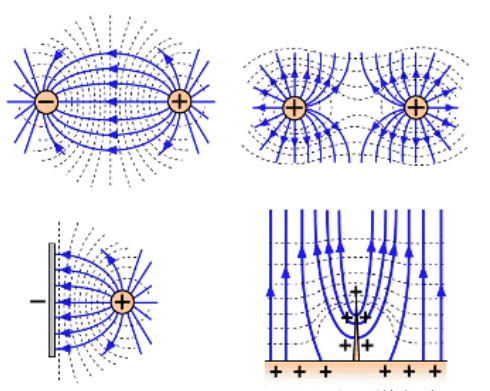
\includegraphics[scale=0.75]{1.png}

\end{document}